\chapter{SOA}
\label{chap:soa}
Der Begriff SOA ist nicht eindeutig definiert. Je nachdem welche Person man in einem Unternehmen fragt, erhält man unter Umständen eine komplett andere Definition. \frqq Die Meisten Definitionen stimmen jedoch zum größten Teil überein und stehen nicht im Konflikt mit einander.\flqq\cite[vgl. Seite 6]{100QA}

Für einen Kaufmann ist SOA etwas anderes als für einen Analysten, damit SOA jedoch verstanden werden kann, werden zunächst einmal einige Definitionen nach \cite{100QA}\ genannt:
\begin{enumerate}
       \item \frqq To the chief information officer (CIO), SOA is a journey that
       promises to reduce the lifetime cost of the application portfolio [...].\flqq \cite[vgl. Seite 6]{100QA}
    
       \item \frqq To the business executive, SOA is a set of services that can be exposed to their customers, partners, and other parts of the organization. Business capabilities, function, and business logic can be combined and recombined to serve the needs of the business now and tomorrow. Applications serve the business because they are composed
       of services that can be quickly modified or redeployed in new
       business contexts, allowing the business to quickly respond to changing
       customer needs, business opportunities, and market conditions.\flqq \cite[vgl. Seite 6]{100QA}
       
       \item \frqq To the business analyst, SOA is a way of unlocking value, because business processes are no longer locked in application silos. Applications no longer operate as inhibitors to changing business needs.\flqq \cite[vgl. Seite 6]{100QA}
       
       \item \frqq To the chief architect or enterprise architect, SOA is a means to
       create dynamic, highly configurable and collaborative applications
       built for change. SOA reduces IT complexity and rigidity. SOA becomes the solution to stop the gradual entropy that makes applications
       brittle and difficult to change. SOA reduces lead times and costs
       because reduced complexity makes modifying and testing applications
       easier when they are structured using services.\flqq \cite[vgl. Seite ]{100QA}
\end{enumerate}
Jeder der genannten Rollen hat eine eigene klare Definition von dem was SOA ist. Jeder der Definitionen ist jedoch nur ein Teil dessen für was SOA verwendet werden kann. Denn SOA ist eine Herangehensweise und kein festes Modell.

\section{Grundlagen}
\label{sec:Grundlagen}
Das Ziel von SOA ist nicht die Entwicklung zu vereinfachen oder voran zu bringen. SOA soll die Unternehmensweiten Geschäftsprozesse standardisieren und vereinheitlichen. Aus diesem Grund sollte SOA nicht als Modell, sondern als Herangehensweise verstanden werden.
\\\\
Bei der Vereinheitlichung und Standardisierung spielt die Wertschöpfungskette eine wichtige Rolle, da diese die Geschäftsprozesse miteinander verbindet.
\\\\
Bei der Vereinigung verschiedener Geschäftsprozesse spielt die Kommunikation ebenfalls eine entscheidende Rolle. Wie in Kapitel \secref{subsec:conway}\ erwähnt, können nur solche Systeme entworfen werden, welche die Kommunikationsstrukturen der Organisation abbilden. Daher muss, wenn man SOA verwenden möchte, die nötigen Kommunikationswege geschaffen werden, um eine ordnungsgemäße und standardisierte Kommunikation zu gewährleisten.
\\\\
SOA soll zudem dabei helfen Geschäftsprozesse und Geschäftskomponenten in ein bestehendes Unternehmen einzubinden. Als Beispiel die \textit{Auktionen GmbH}\ übernimmt das Unternehmen \textit{Handel GmbH}. Beide Unternehmen besitzen zwar ähnliche Prozesse und Komponenten, können jedoch nicht ohne weiteres in die bestehende Struktur übernommen werden. Mit Hilfe von SOA soll dies vereinfacht werden.

\subsection{Business und IT}
\label{subsec:BusinessAndIT}
Ein Zentraler Bestandteil von SOA ist die IT. IT darf nie zum selbst Zweck existieren. Sie wird immer zur Unterstützung der Geschäftsprozesse eingesetzt. Umso mehr Geschäftsprozesse existieren, umso mehr Software existiert in einem Unternehmen.
\\\\
Oft existieren bereits verschiedene Anwendungen wie ERP- oder COBOL-Systeme. Mit SOA soll dafür gesorgt werden, das diese Systeme möglichst effizient miteinander arbeiten können.
\begin{quotation}
    \frqq The complexity of the technology infrastructure at many companies in the financial services sector makes it very hard to leverage IT services in a coordinated way across the enterprise. Many large companies have either merged or acquired other very large companies resulting in the integration of new business units with very different work cultures and widely different information infrastructurse. The need to be able to trust and understand the information about the business across its many disaggregated parts has been a prime motivator for change in the IT infrastructure at these companies.\flqq \cite[S. 17]{SOAForDummies}
\end{quotation}

Mit SOA wird die IT-Infrastruktur eines Unternehmens in zwei Teile geteilt. Auf der einen Seite existiert die Geschäftsschicht mit der Geschäftslogik und auf der anderen Seite die IT-Schicht, welche die Computing-Ressourcen verwaltet. Durch diesen Aufbau ist es nicht nötig, das ein Business Manager die IT-Schicht verstehen muss.
\\\
In der Geschäftsschicht sind nur Dienste, mit denen Kunden, Lieferanten und Business Partner interagieren. Diese Personen benötigen, genauso wie ein Business Manager, keine Wissen darüber, was in der IT-Schicht existiert oder wie diese aufgebaut ist. Andersherum sind in der IT-Schicht nur Dienste und Applikationen vorhanden, wofür die IT-Abteilung zuständig ist.
\\\\
Damit diese Schichtentrennung funktioniert, wird darauf geachtet, dass in der Geschäftsschicht möglichst wenig Komplexität nach außen sichtbar ist.

\subsection{Unternehmens Komponenten}
\label{subsec:UnternehmensKomponenten}
Dazu müssen zunächst einmal alle Komponenten eines Unternehmens identifiziert werden. Die nachstehende Abbildung (\ref{fig:UnternehmensKomponenten}) zeigt ein Beispiel dieser Identifizierung:

\begin{figure}[htb]
    \centering 
    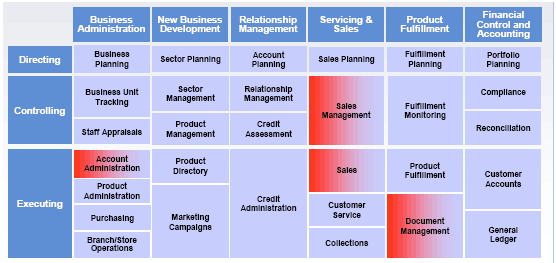
\includegraphics[width=\linewidth]{content/images/UnternehmensKomponenten}\
    \quelle\url{http://www.jot.fm/issues/issue_2008_05/column5/}
    \caption[Unternehmens Komponenten]{Unternehmens Komponenten\\}
    \label{fig:UnternehmensKomponenten}  
\end{figure} 
\newpage
Aus diesen Komponenten müssen nun die Geschäftsprozesse identifiziert werden, beginnend mit den wichtigsten. Daraus ergeben sich anschließend die Komponenten, welche unter einander kommunizieren müssen. Die in der Abbildung Rot dargestellten Komponenten sind schließlich das Resultat aus der Analyse. Hat man die Komponenten über Kommunikationswege verbunden, werden die nächsten Geschäftsprozesse identifiziert. Diese Prozedur wird solange wiederholt, bis alle Komponenten mit einander verbunden sind.

\section{Architektur}
\label{sec:SoaArchitektur}
Die Architektur in einem SOA-System unterliegt dem Paradigma einer "`Service-orientierten Architektur"'. Mit diesem Paradigma ist der Begriff \textit{Dienst} verbunden. Dieser ist im Falle von SOA jedoch zunächst nicht richtig, denn Anwendungen wie ERP- oder COBOL-Systeme sind eigenständige Anwendungen und keine Dienste.
\\\\
Damit eine ERP-Anwendungen ihre Funktionalitäten bereitstellen kann, muss ein Adapter erstellt werden. Dieser Adapter stellt die Funktionalität in Form von Schnittstellen bereit und kann als Dienst bereitgestellt werden. Der Adapter übernimmt dabei Aufgabe wie Fehler abzufangen und die Daten in angemessener Weise aufzuarbeiten, damit diese über die jeweilige Schnittstelle abgerufen werden können, sowie die eigentliche Anwendung zu steuern.
\\\\
Schnittstellen können dabei HTTP-Rest oder SOAP sein. Es ist jedoch auch Möglich weitere Schnittstellentechnologien zu verwenden, wie RMI. Genauso kann es möglich sein "`Message Oriented Middleware"' zu verwenden, um Informationen bereit zu stellen.

\section{Enterprise-Service Bus - ESB}
\label{sec:esb}
Der Begriff "`Enterprise-Service Bus (ESB)"' wird oft im Zusammenhang mit SOA verwendet. Der ESB ist jedoch kein Teil von SOA, sondern nur ein Mittel zum Zweck, um die Kommunikation zu vereinheitlichen. Der Enterprise-Service Bus dient dabei als Nachrichten Komponente, welcher die Nachrichten entgegen nimmt und an die jeweiligen Empfänger weiterleitet, sowie als Transformator von Nachrichten, um Interoperabilität zu schaffen. Außerdem kann der ESB häufig als \textit{Service Discovery} eingesetzt werden. Jedoch kann diese Aufgabe auch von einer eigenständige Anwendung, wie \textit{Zookeeper} oder \textit{Consul}, übernommen werden.
\\\\
Grundsätzlich wird ein ESB eingesetzt, um an einer zentralen Stelle die Kommunikation zu steuern und die Geschäftsprozesse abzubilden. Am einfachsten lässt sich das an einem Beispiel erklären.
\\
Man Stelle sich eine Banking-Anwendung vor, an der man sich anmeldet. Es werden daraufhin folgende Informationen angezeigt:

\begin{enumerate}
    \item Name
    \item Kontostand
    \item EC- und Kreditkarten
    \item Liste der Aktienfonds
\end{enumerate}

Jede Information stammt aus einem anderen Teil des Systems und werden von verschiedenen Anwendungen über Schnittstellen bereitgestellt. Die Schnittstellen können sich dabei von Anwendung zu Anwendung unterscheiden. So kann zum Beispiel eine Anwendung die Informationen über HTTP bereitstellen, während eine andere sie über SOAP bereitstellt. So können die Informationen zum Beispiel aus einem CRM-System (Kundenbeziehungsmanagement-System) stammen oder durch PHP oder Ruby erzeugt werden.

Anders als man jedoch vermuten würde, lässt man die Oberfläche, bzw. das System, nicht direkt mit den einzelnen Komponenten reden. Die gesamte Kommunikation läuft dabei über den \textit{Enterprise Service Bus} ab. Nachstehende Abbildung soll dies genauer erläutern:

\begin{figure}[htb]
    \centering 
    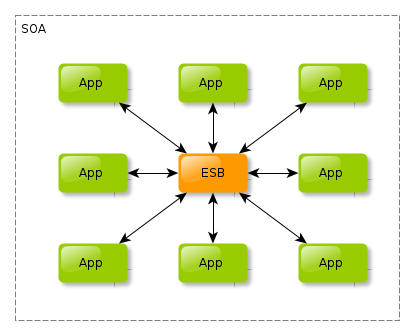
\includegraphics[width=\linewidth]{content/images/esb-ok}\
    \caption[ESB]{Enterprise Service Bus}
    \quelle\url{https://zato.io/docs/intro/esb-soa-de.html}
    \label{fig:esb}  
\end{figure}
\newpage
Benötigt eine Anwendung (in der Abbildung App genannt) Informationen, konsultiert diese zunächst den ESB. Der ESB kennt die anderen Anwendungen oder benutzt einen Dienst, welcher die Informationen bereitstellen kann, und stellt daraufhin die angeforderten Informationen bereit. Dabei ist es egal wo die Dienste liegen, solange sie über das Netzwerk ansprechbar sind.